\section{Stereotyp / Keyword}

\begin{tcolorbox}[title=Konzept der Stereotypen]
    \textbf{Stereotypen} erlauben es, existierende Modellelemente mit einer zusätzlichen Semantik zu versehen. \\
    Die Bezeichner von Stereotypen werden in \textit{Guillemots} (\guillemotleft \guillemotright) gesetzt.\\

    \noindent
    Die UML erlaubt durch vordefinierten \textbf{Keywords} die Unterscheidung von Modellierungskonzepten mit gleicher grafischer Notation.  bspw. \guillemotleft enumeration\guillemotright um zu verdeutlichen, dass es sich bei einem Modellelement um eine Aufzählung handelt (vgl.~\cite[28]{Bal05}).
\end{tcolorbox}


\begin{figure}
    \centering
    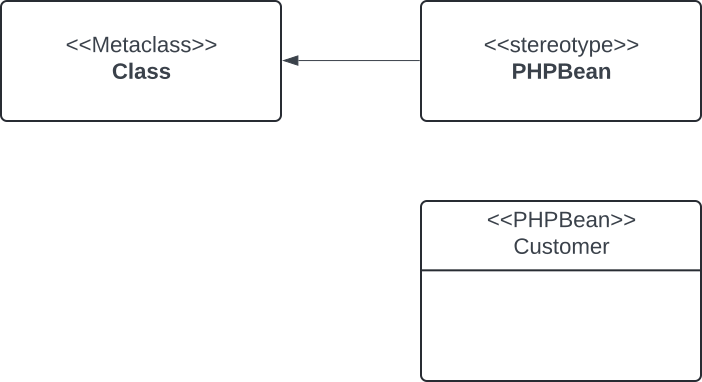
\includegraphics[scale=0.4]{chapters/Anhang/CheatSheets/SE3/img/stereotyp}
    \caption{
        Definition eines Stereotyps \textit{PHPBean} als Erweiterung des UML Konzepts \textbf{Class} (oben) und Verwendung unter der Notation von Klassendiagrammen (unten).
        Vgl. S.177, \url{https://www.omg.org/spec/UML/2.4.1/Infrastructure/PDF} , abgerufen 22.06.2024. Zur Notation von \textit{Extensions} s.a. ebenda, S.179.
        (Quelle: eigene)
    }
\end{figure}



